\documentclass[10pt]{article}
\usepackage[a4paper,margin=17mm]{geometry}
\usepackage{graphicx,hyperref,booktabs,amsmath}
\hypersetup{colorlinks=true,urlcolor=blue}
\setlength{\parindent}{0pt}\setlength{\parskip}{5pt}
\begin{document}
\begin{center}\Large One-pass affine consequences\\[3pt]
\normalsize Coefficient certificates and a fixed-input null result --- 16 November 2026\end{center}
The Rust compiler appends affine consequences and substituted quadratic
residuals while retaining every original variable and equation. A separate
BigUint coefficient checker checks row lineage and exact identities before
constructing the admitted output. Core PCC-20261116-313284; corrected shell
interface PCC-20261116-503900. All standing unsigned/unverified. [pcc:unverified]

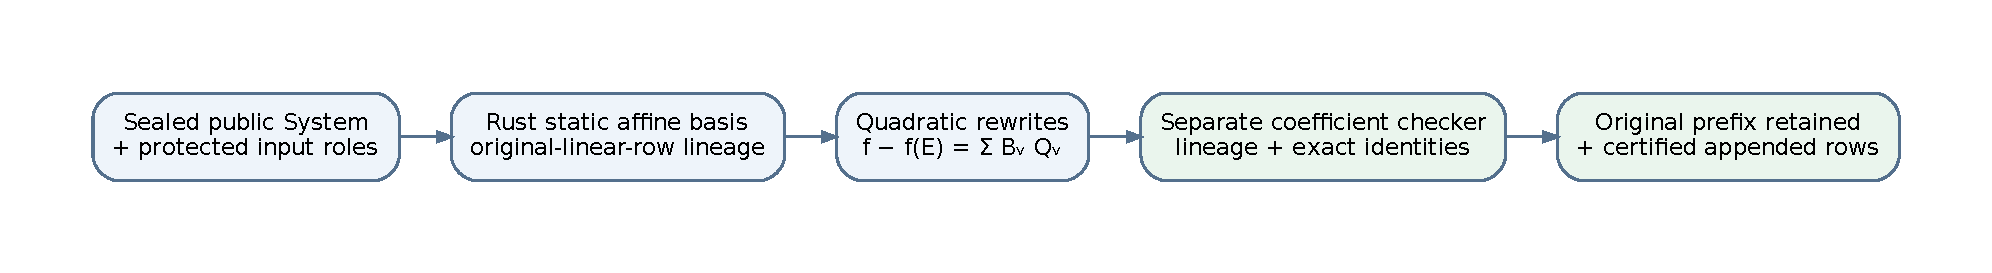
\includegraphics[width=\linewidth]{pipeline.pdf}
For each pivot, $B_v=x_v-E_v$ is a constant linear combination of original
linear rows. The checker tests $f-f(E)=\sum_v B_v Q_v$ coefficient by
coefficient. Semantic branching inputs are protected from pivoting;
protected-only side consequences remain. One static pass, no variable
removal, no branch-local elimination or F4. [pcc:unverified]

\begin{center}\begin{tabular}{lrr}\toprule
Fixed curve inputs & Before $\to$ after outcome & Nodes before $\to$ after\\\midrule
Toy original, 13 targets & Unsupported $\to$ Unsupported & $511\to511$ each\\
Toy indexed, same 13 & Root $\to$ Root & unchanged, see graph\\
Actual-q1 original/indexed, two & Root $\to$ Root & $8\to8$ each\\\bottomrule
\end{tabular}\end{center}
All 28 curve requests retain outcome class and node count. This is a null
result for branch counts of this static pass on these inputs. It establishes
neither equal decision traces nor complete work, time or memory. Returned
roots pass independent original-equation and native indexed-row/group replay.
[pcc:unverified]

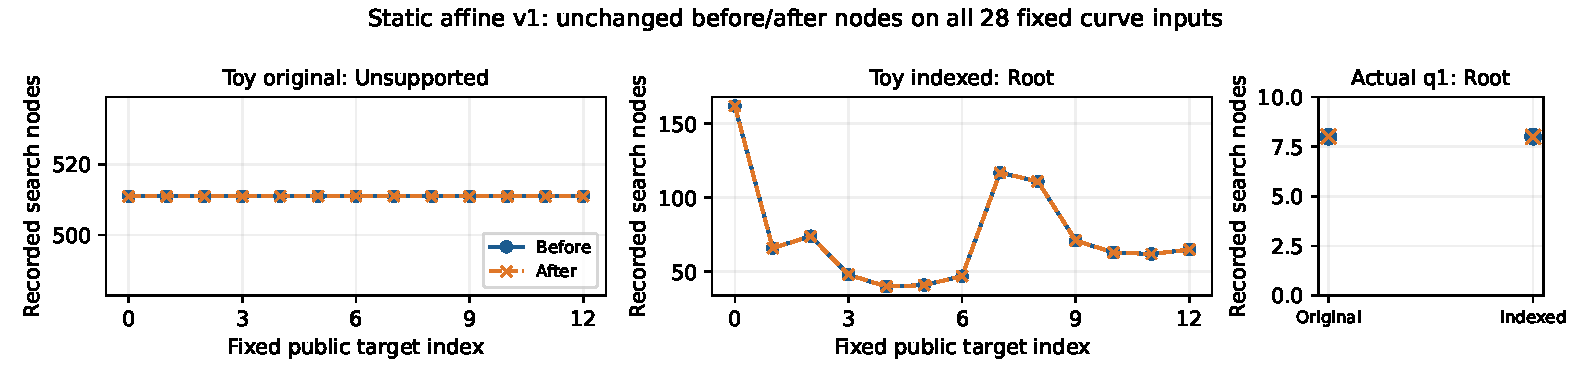
\includegraphics[width=\linewidth]{nodes.pdf}
Recorded values for all 28 inputs, no sampling or uncertainty model. The
indexed toy sequence is 162, 66, 74, 48, 40, 41, 47, 117, 111, 71, 63, 62, 65 in both arms.
These are partial diagnostics, not a speed or total-work comparison.
[pcc:unverified]

\textbf{Huge actual inputs: static coefficient checks only.}
\begin{center}\begin{tabular}{lrrrr}\toprule
Input & Variables retained & Equations before/after & Pivots & Solver calls\\\midrule
Original &1059&1089/1174&37&0\\
Indexed &1989&2223/2548&157&0\\\bottomrule
\end{tabular}\end{center}
Degree remains two; all original constraints stay. Compiler reservation/event
counters are partial, and cumulative modeled bytes are not live storage/RSS.
[pcc:unverified]

\textbf{Domain.} Toy p101/A95/h(17,12)/a17/q3/k8, arity two, distinct raw
columns, aliases retained, identity columns excluded. Distinct actual control:
$p=2^{255}-19$, A486662, $h_{new}=h_{old}^{213156431}$, a60824497/q1/k2, arity two.
It has TWO columns, not the huge original q213156431 base. [pcc:unverified]

\newpage
\begin{center}\Large Controls, source identity and next check\end{center}
\textbf{Coverage.} All 34 sealed quadratic requests have checked certificates:
26 toy, two actual-q1, two huge static and four small polynomial inputs.
Fp29 truth controls inspect 24,389 assignments/one accepted (coupled three
variables), and 841 each for conflict/zero accepted, nonlinear/28 accepted
and protected/one accepted. Coupled Unsupported becomes Root; conflict
Unsupported becomes NoRootObservation; nonlinear remains Unsupported, which
is not an absence certificate. Eight corrupted certificates, original binding
mutation, 11 malformed requests, oversized input and seven forced caps stay
in raw evidence. The old Unsupported-child/other-child root regression is a
separate declared degree-four old-interface control. [pcc:unverified]

\textbf{Failed path and launcher correction.} First release unit controls
passed with an unused import warning. A later strict-Clippy iterator-style
failure and source remain; final release build/fmt/strict all-target Clippy
pass locally. No Rust/fixture change followed qualification. The initial
standalone interface calls used a Python launcher, contrary to repository
rules. Those receipts remain unchanged and are excluded from final interface
acceptance. A separately frozen thin shell reran the identical three positive
and ten negative coefficient-file checks, all with expected exits. No solver
discovery rerun. See \path{INTERFACE_PROVENANCE.md}. [pcc:unverified]

\textbf{Frozen evidence.} Composite 64-input source: unchanged 43-input v2
archive +six-input indexed delta +six-input worklist delta +nine-input affine
delta (53,152 bytes). No monolithic archive is claimed. All source pins,
four archive round-trips and nine compiled-in bindings matched. Separate
2,710,656-byte executable SHA-256:\\
\texttt{54ad26145290b1228e4f45c6669176ae4b79ca17c7f187441bc9b6c2b7d1de7d}.
[pcc:unverified]

Complete core raw evidence is 283 files/16,263,777 bytes, one 146,256-byte
archive SHA-256:\\
\texttt{ef5b561a184672f36ac9c2e12963f23d14d56aa731ea6e3d79f68968b3e2a875}.
The corrected shell round is separate, 1,576 bytes. Local raw bytes are
retained. The core archive needs a genuine trusted artifact-store receipt;
source publication alone is not upload success. See \path{PUBLISHING.md},
\path{FROZEN.md}, \path{REPRODUCE.md}, manifests and pre-call receipts in
\path{affine-closure-v1/}. [pcc:unverified]

\textbf{Prior art.} Shoup, \emph{A Computational Introduction to Number Theory
and Algebra}, v2, section14.4, pp388--391, elementary row operations and
elimination: \url{https://shoup.net/ntb/ntb-v2.pdf}.
Repository affine-substitution predecessor:
\path{research/p256_aux_smooth_20261114/continuation_20261116/REPORT.md}
and \path{linear_reduce.cpp}. Mackworth1977 scheduling informs the unchanged
worklist solver. No novelty for linear elimination or telescoping identities.
KB tools/wrapper unavailable; Magma handbook returned401 and was not read.

\textbf{Acceptance boundary.} Public input sealing, literal original prefixes,
certificates and fixed controls are implemented with native unsigned evidence.
Formal/signed compiler and execution validation, full cold cost/live memory,
huge original-base root discovery and useful-yield/family/selection/kernel/
recovery bridges remain open. Prime-field validity for solving is external.

\textbf{Next discriminating implementation.} A separate versioned branch-local
affine reducer can expose equations becoming linear after assignments. Retain
lineage, exact rewrite certificates and basis rollback; compare the same public
inputs/root order/limits. It may prune branches or reproduce this null result
with extra bookkeeping. Price parsing, compilation, certificate work,
normalization, BigUint/container allocation, live storage, every failed branch,
selection, replay and serialization before a performance comparison. The CI
checker schedules none of this work. Canonical cost/exponent charts and
benchmarks stay unchanged: no admitted performance datum is added.
Original criteria/source pins remain unchanged. [pcc:unverified]
\end{document}
